% Chapter 1

\chapter{Simulation and Results} % Main chapter title

\label{simulacra} % For referencing the chapter elsewhere, use \ref{Chapter1} 

\lhead{Simulation and Results} % This is for the header on each page - perhaps a shortened title

%----------------------------------------------------------------------------------------

\section{Simulator used}
Write in detail about Castalia - justify use of Castalia

% Add Param table

\section{Performance Evaluation}

%Write about Simulation scenario

For evaluating the performance of DS-MMAC, we have compared the results of the proposed approach with Hybrid MAC\cite{hmac}. Simulation is done in Castalia, an omnetpp based framework for low power networks with realistic radio propagation models and analysis tools \cite{castalia}. The parameters chosen for comparison are listed in Table \ref{sim_para}.

We have considered a simulation area of $100 \times 100m$ where an unstructured deployment of sensor node is done. The mobile nodes are initially distributed evenly across the simulation area. The mobile nodes follow the Random Waypoint mobility model and move at a constant velocity. The simulation was run for 1000 seconds. Simulation was done by varying the number of mobile nodes and by varying the velocity of the node.


\begin{table}[h]\scriptsize
\begin{center}
\caption{Simulation Parameters}
\label{sim_para}
    \begin{tabular}{ | l |p{3cm} |}
    \hline
Parameters & Values \\  \hline
Network Size & $100 \times 100 $ $m^2$ \\ \hline
Number of Static Nodes & $25$ \\ \hline
Communication radius & $30m$ \\ \hline
Velocity & 2m/s \\ \hline
Number of Mobile Nodes & 1 to 70 \\ \hline
Packet size & 128byte \\ \hline
Simulation Time & 1000Sec \\ \hline
    \end{tabular}
\end{center}
\end{table}


Network lifetime is the deciding factor in any network protocol design in Wireless Sensor Networks. Energy consumption of the proposed protocol was compared against the Hybrid MAC protocol. The results plotted in Figure \ref{fig:em} was done by changing the number of mobile nodes from one to fifteen with a velocity value 2m/s. From the results, it is observed that the power consumption of mobile nodes in our approach is substantially lower than that of Hybrid MAC. This is because of the increase sleep time of mobile nodes in the DS-MMAC approach.\\
\begin{figure}[h]{} 
  \begin{center}
		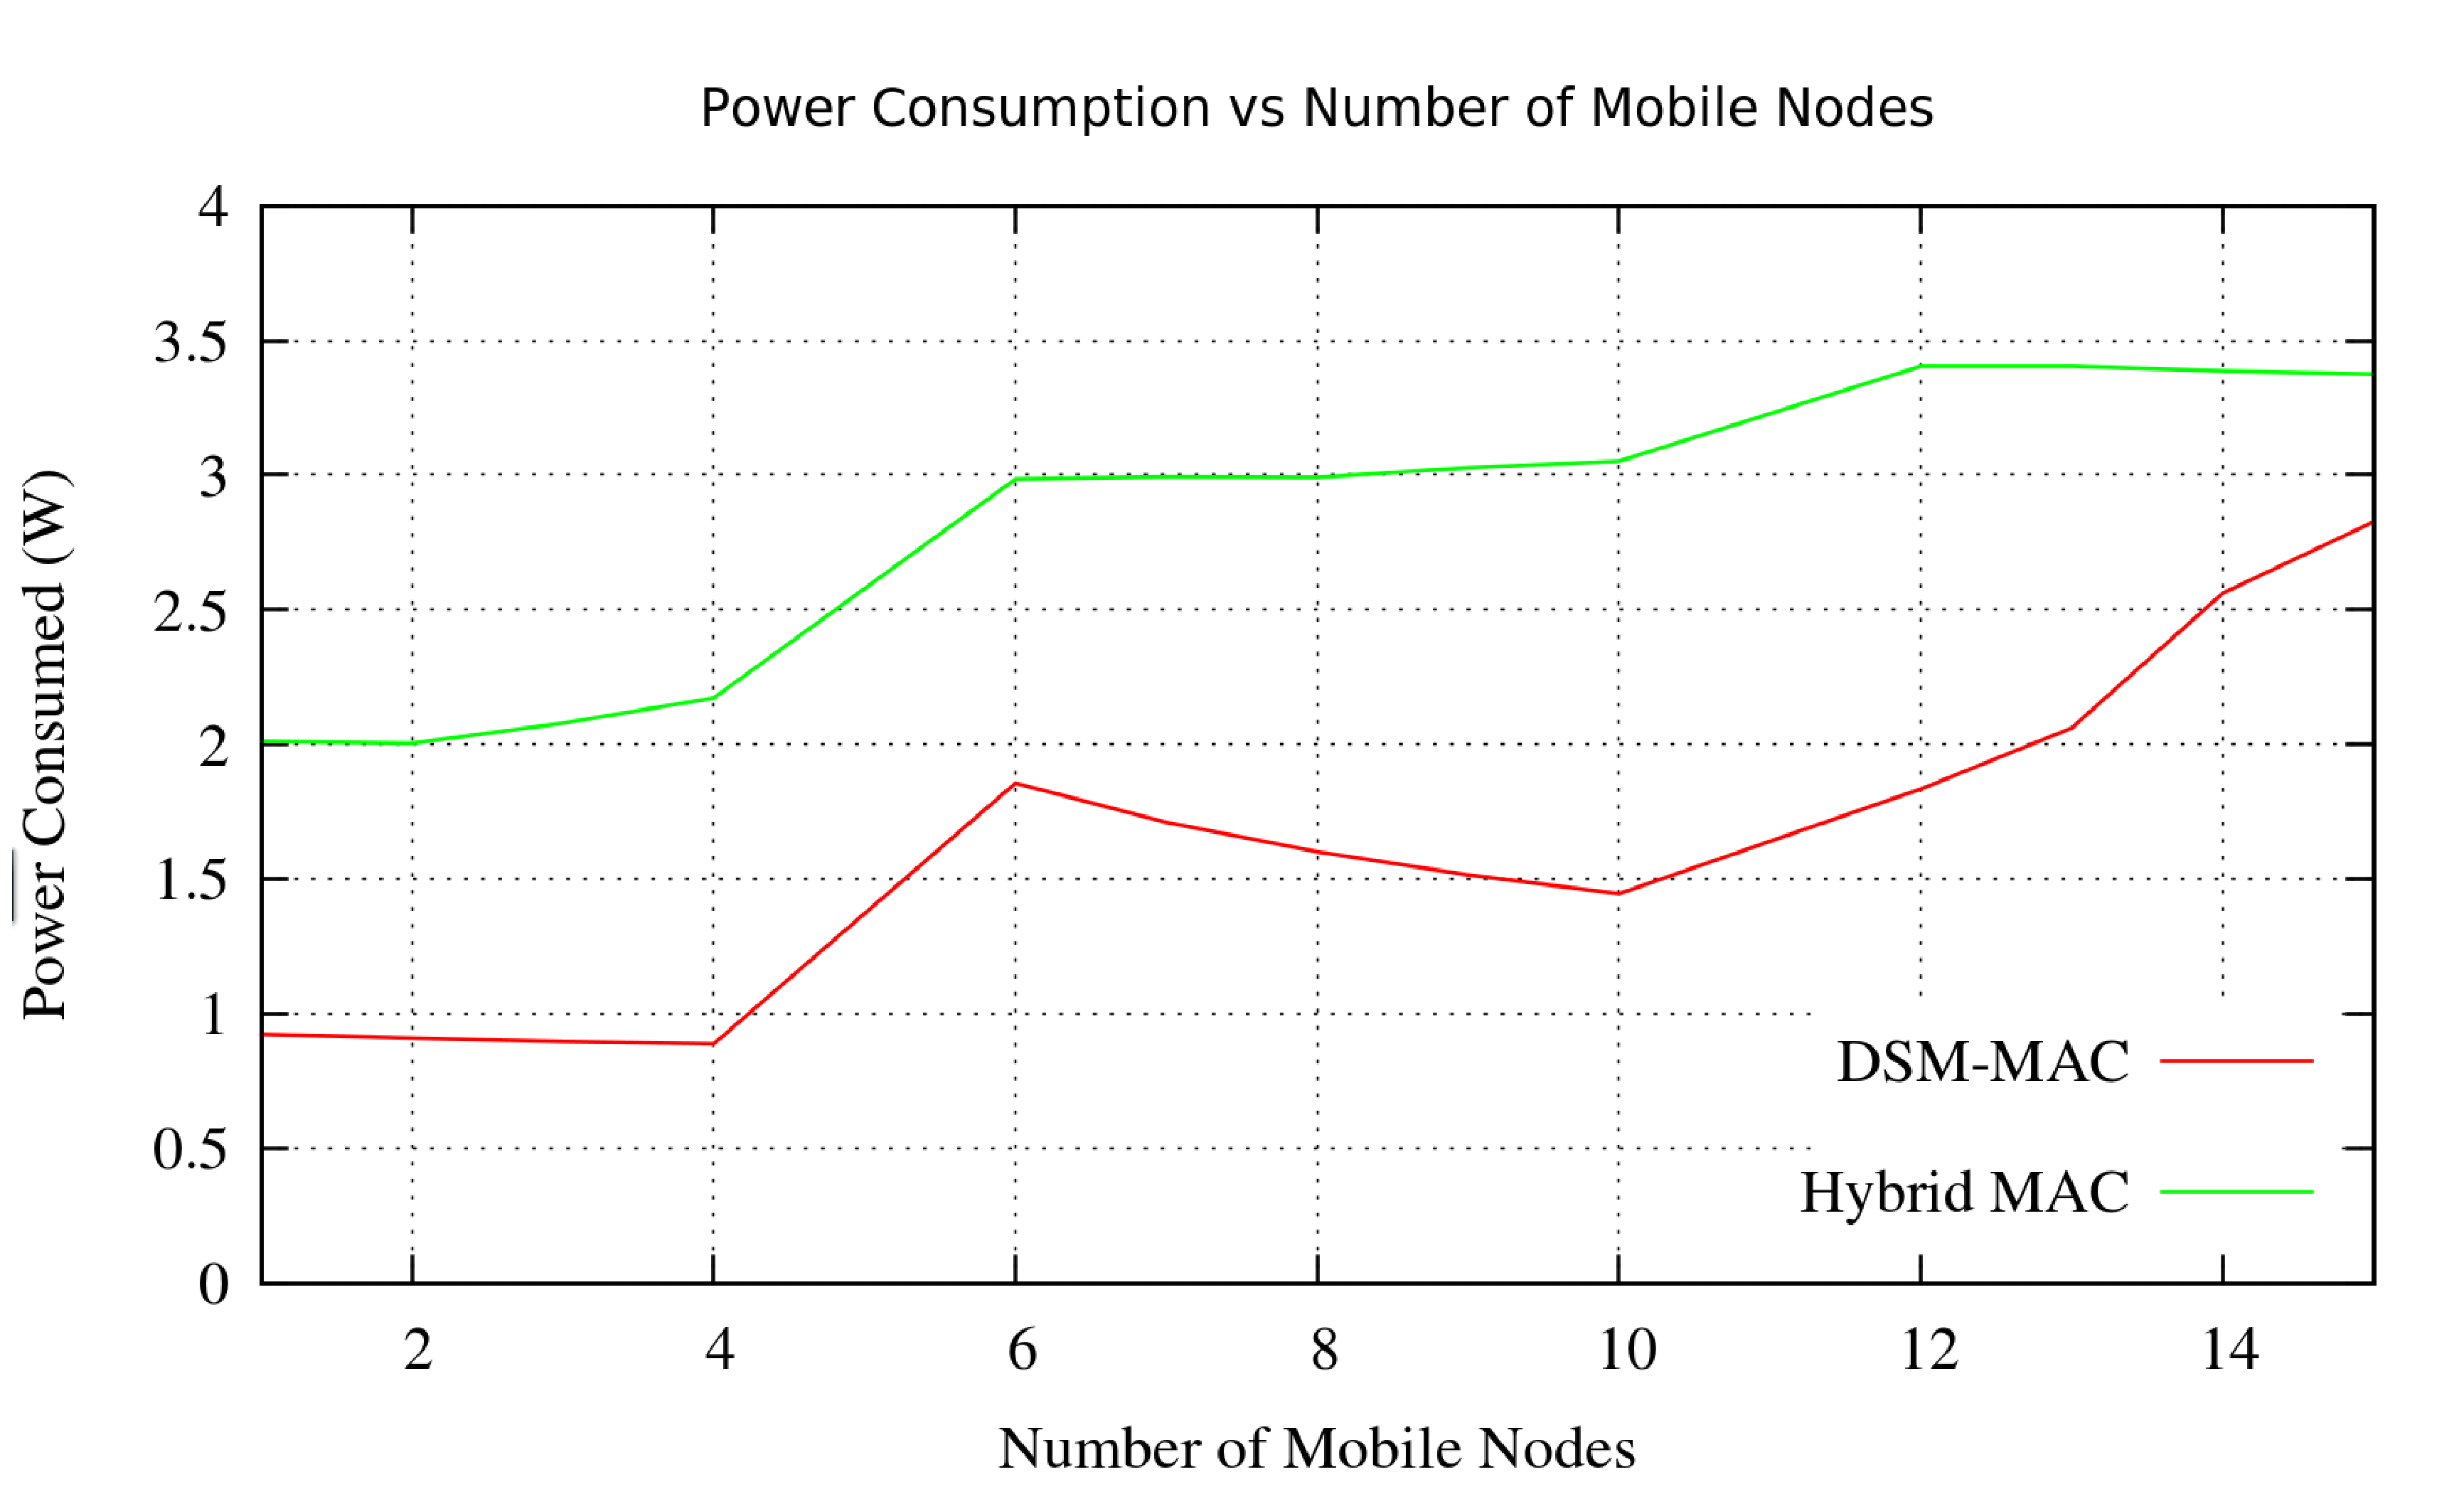
\includegraphics[ width=8.5cm,height=6cm]{em}
  \end{center}
	\caption{Power Consumption vs Number of Mobile Nodes}
		\label{fig:em}
\end{figure}

The Packet delivery ratio is basically the ratio of the number of packets sent to the number of packets received. Figure \ref{fig:PDR} shows the difference in delivery ratio w.r.t to the number of mobile nodes.  Simulation is done for a maximum of 70 mobile nodes.  Hybrid MAC protocol performs slightly better when compared to the proposed approach. Since the neighboring clusters operate on the same channel, the channel interference is high and hence the delivery ratio decreases.
\begin{figure}[h]{} 
  \begin{center}
    		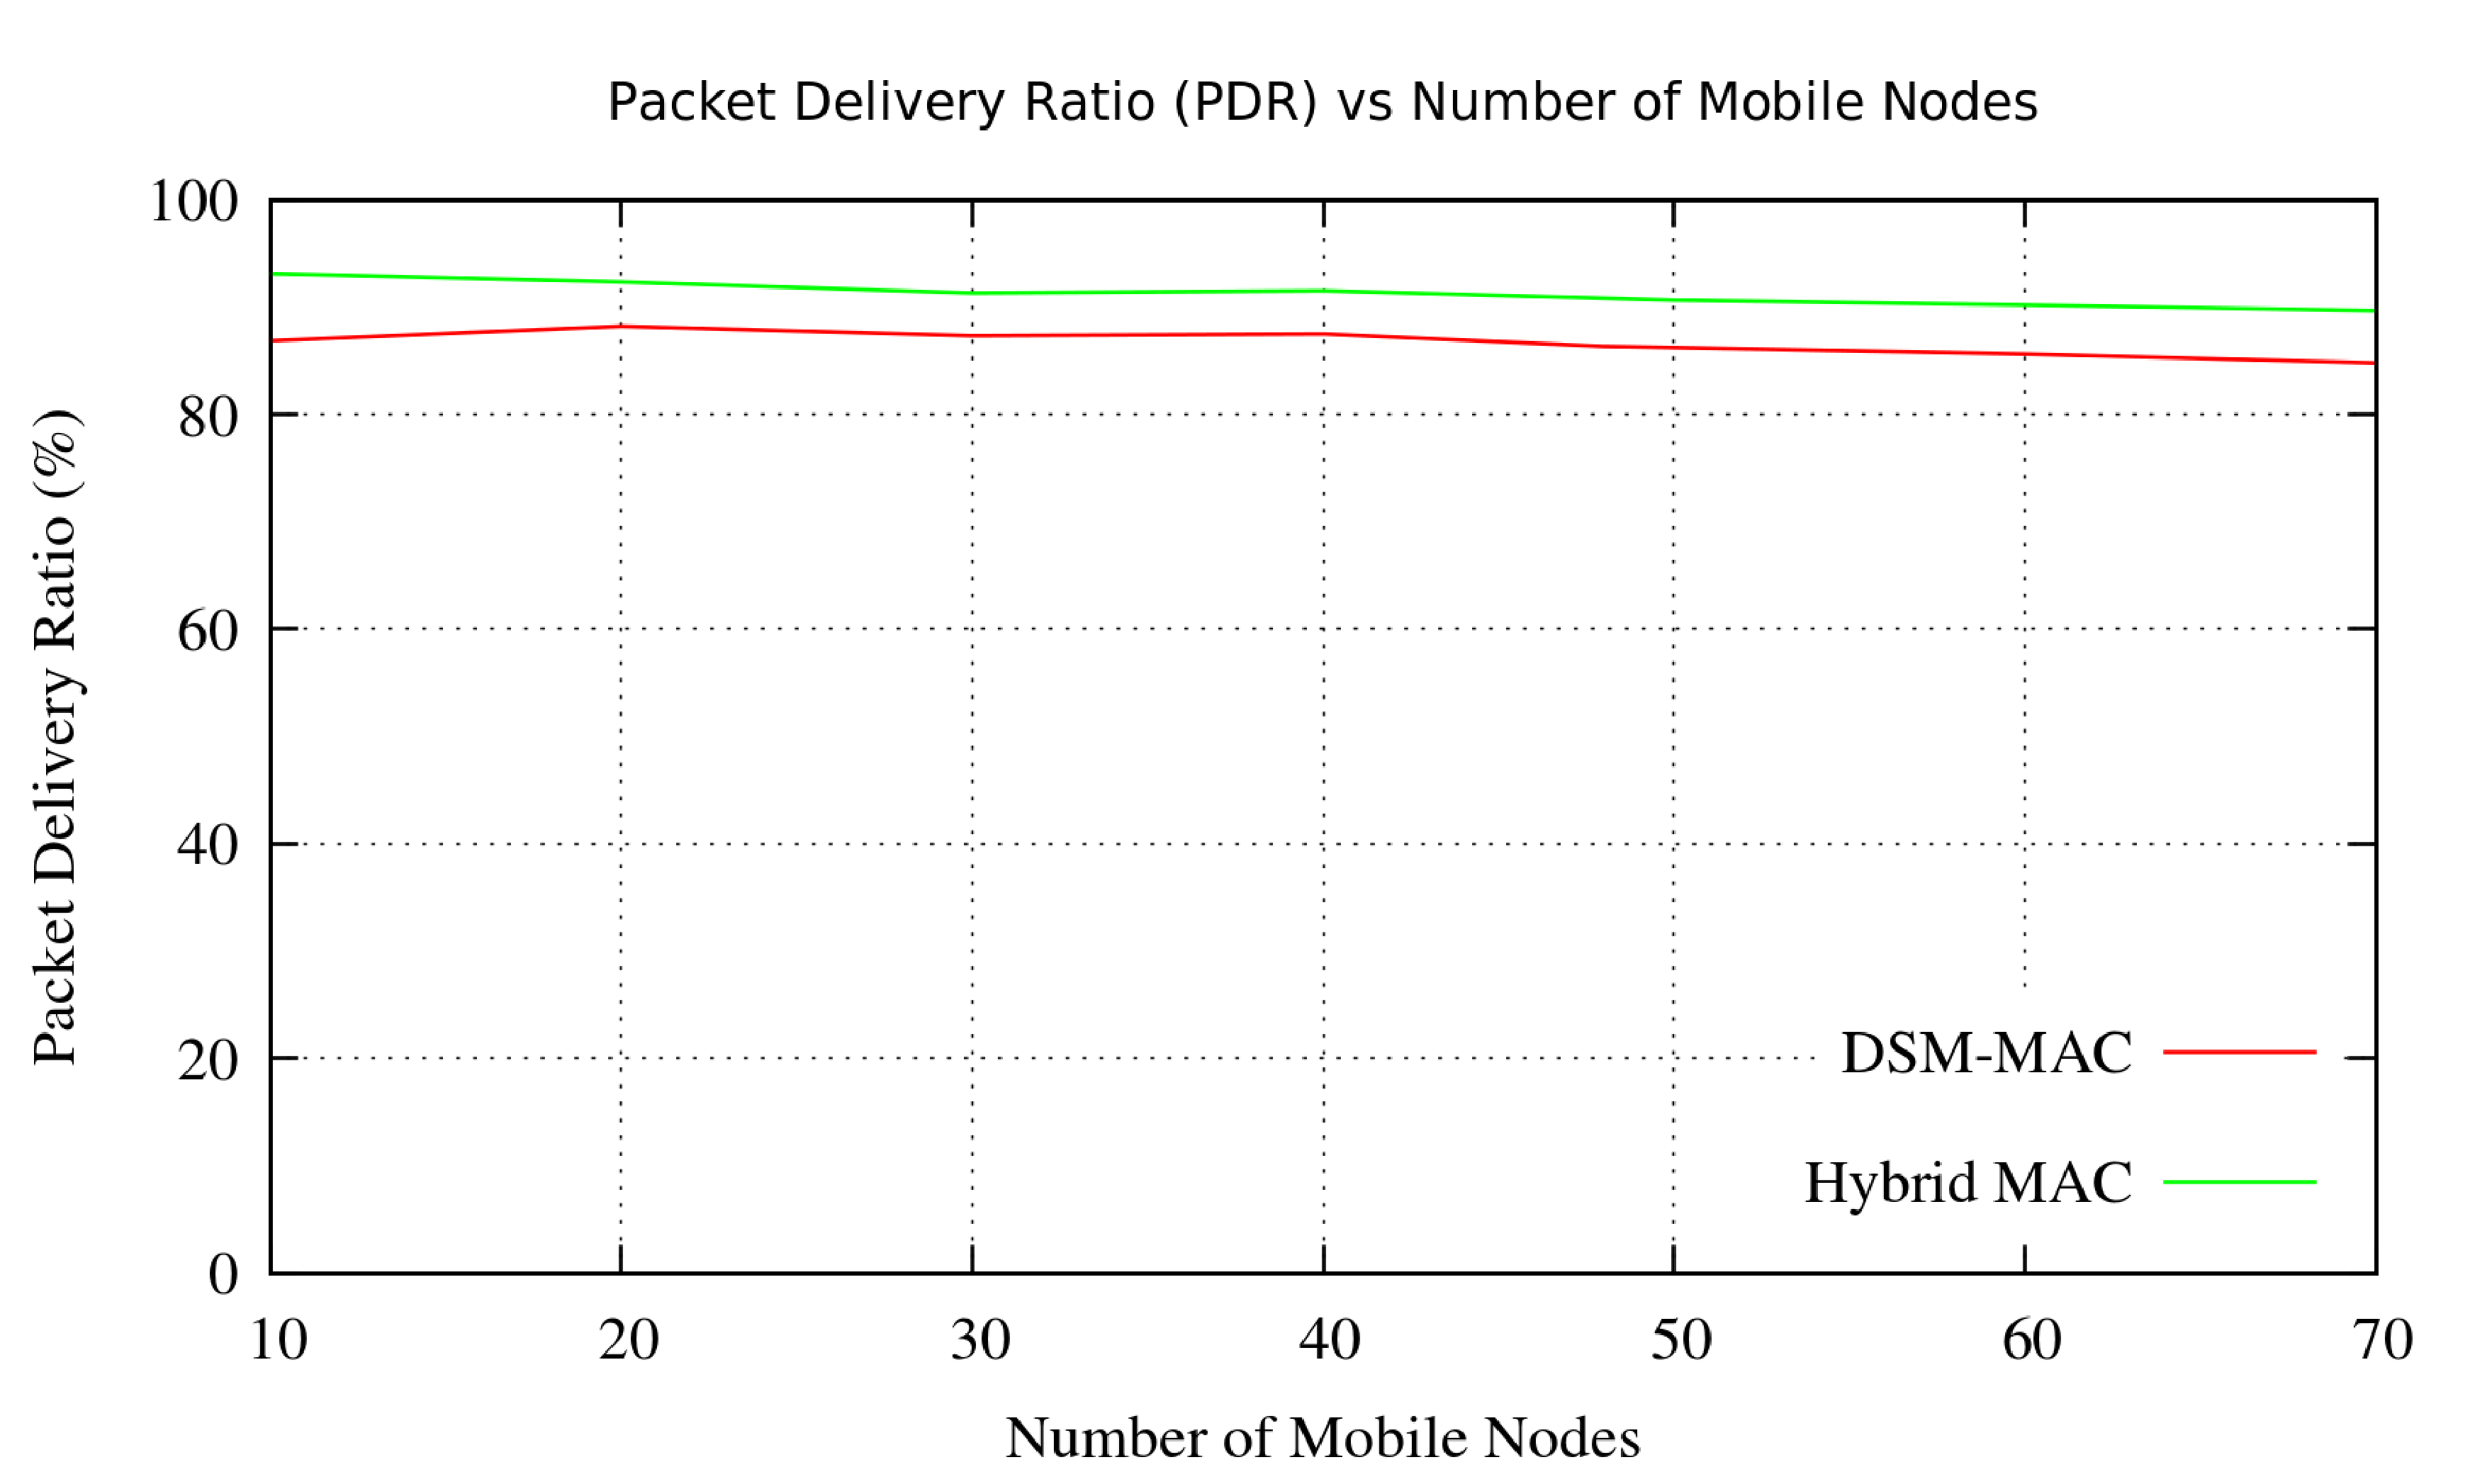
\includegraphics[ width=8.5cm,height=6cm]{prm}
  \end{center}
	\caption{PDR vs Number of Mobile Nodes}
	\label{fig:PDR}
\end{figure}

 Even though the packet delivery ratio is less, the number of packets transmitted and received per second is higher in DS-MMAC approach. This is because of the number of rounds (iteration) per unit time is higher for the same number of mobile nodes. Hence the number of packets send and received per unit time is also higher. This is clear in the Figure \ref{fig:pm}. Figure \ref{fig:pm} shows the relation between the number of packets received per unit time at MAC layer w.r.t the number of mobile nodes. It is clear that the number of packets received is higher in DS-MMAC approach.  But it is a reasonable tradeoff for reduced power consumption and increased throughput. It is a reasonable tradeoff for reduced power consumption and increased throughput. Multichannel based MAC layer implementation for data communication can help in improving the packet delivery ratio.  
 Simulations were done to compare the number of packets delivered w.r.t the velocity of the mobile node. This is done by varying the velocity from $1$ to $10$ m/s. As shown in the Figure \ref{fig:pv}, our approach gives a considerable increase in the number of packets delivered when compared to Hybrid MAC approach. \\

\begin{figure}[h]{} 
  \begin{center}
		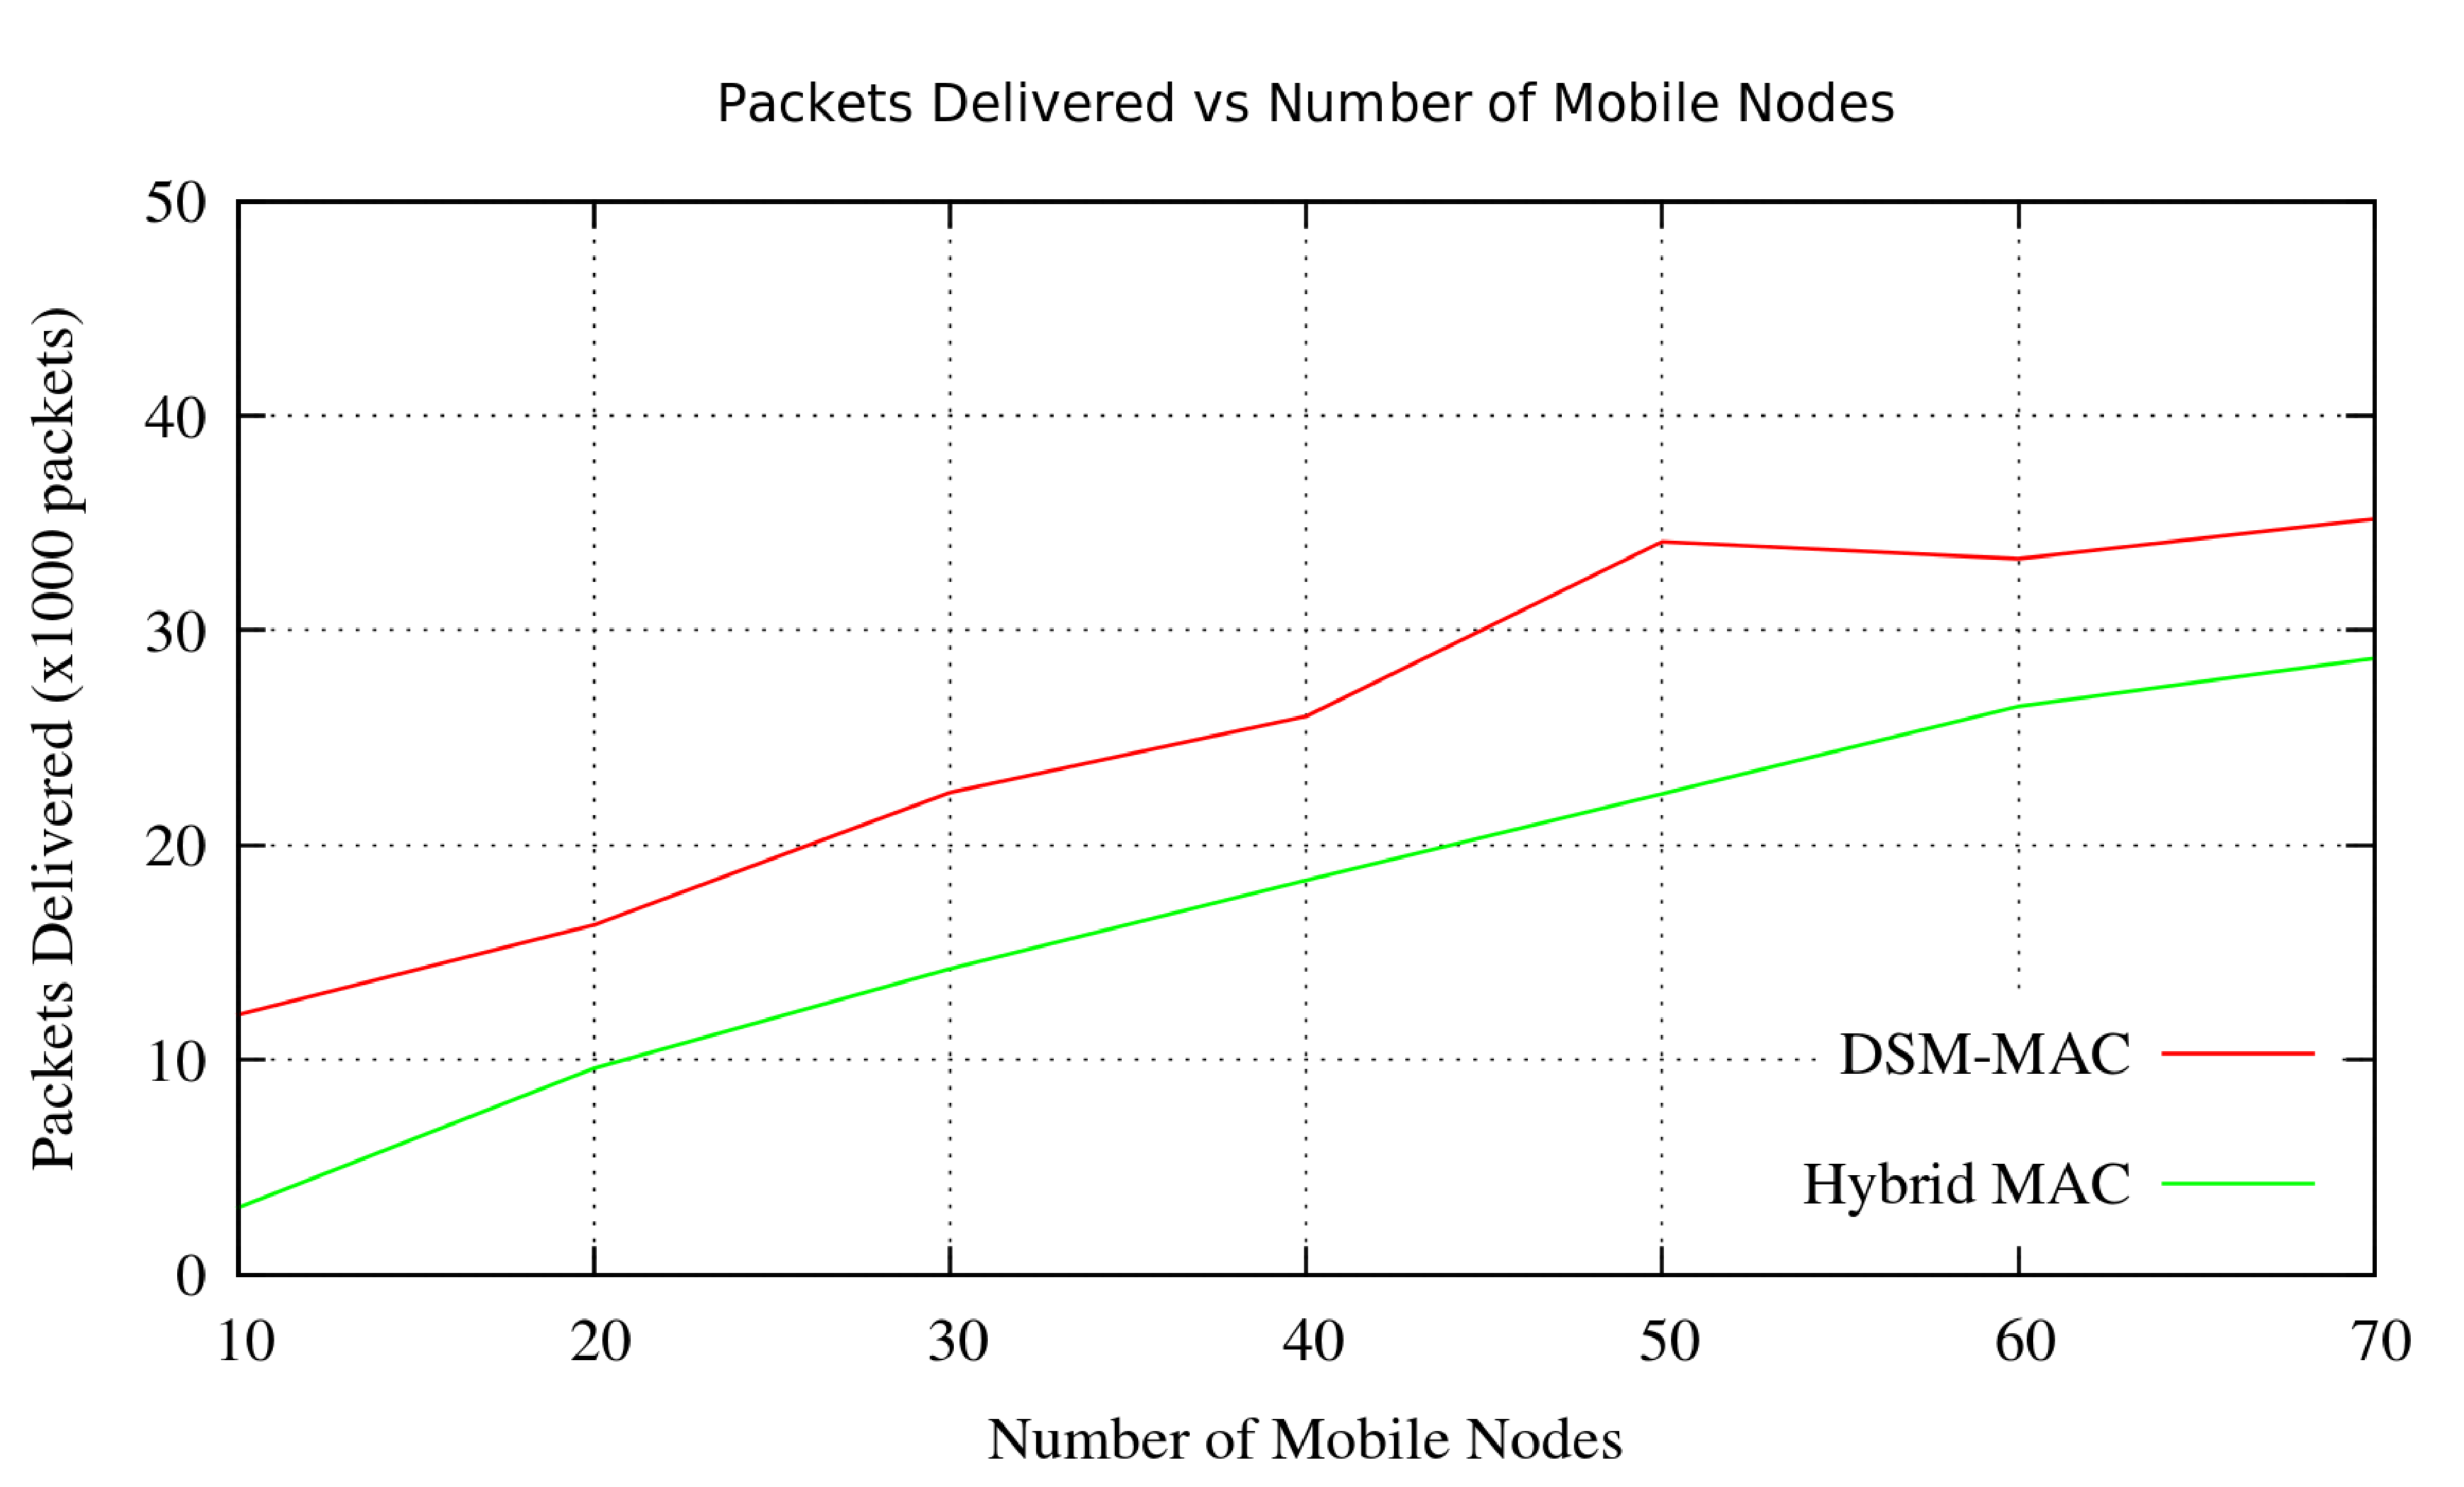
\includegraphics[ width=8.5cm,height=6cm]{pm}
  \end{center}
	\caption{Packets Delivered vs Number of Mobile Nodes}
		\label{fig:pm}
\end{figure}

\begin{figure}[h]{} 
  \begin{center}
		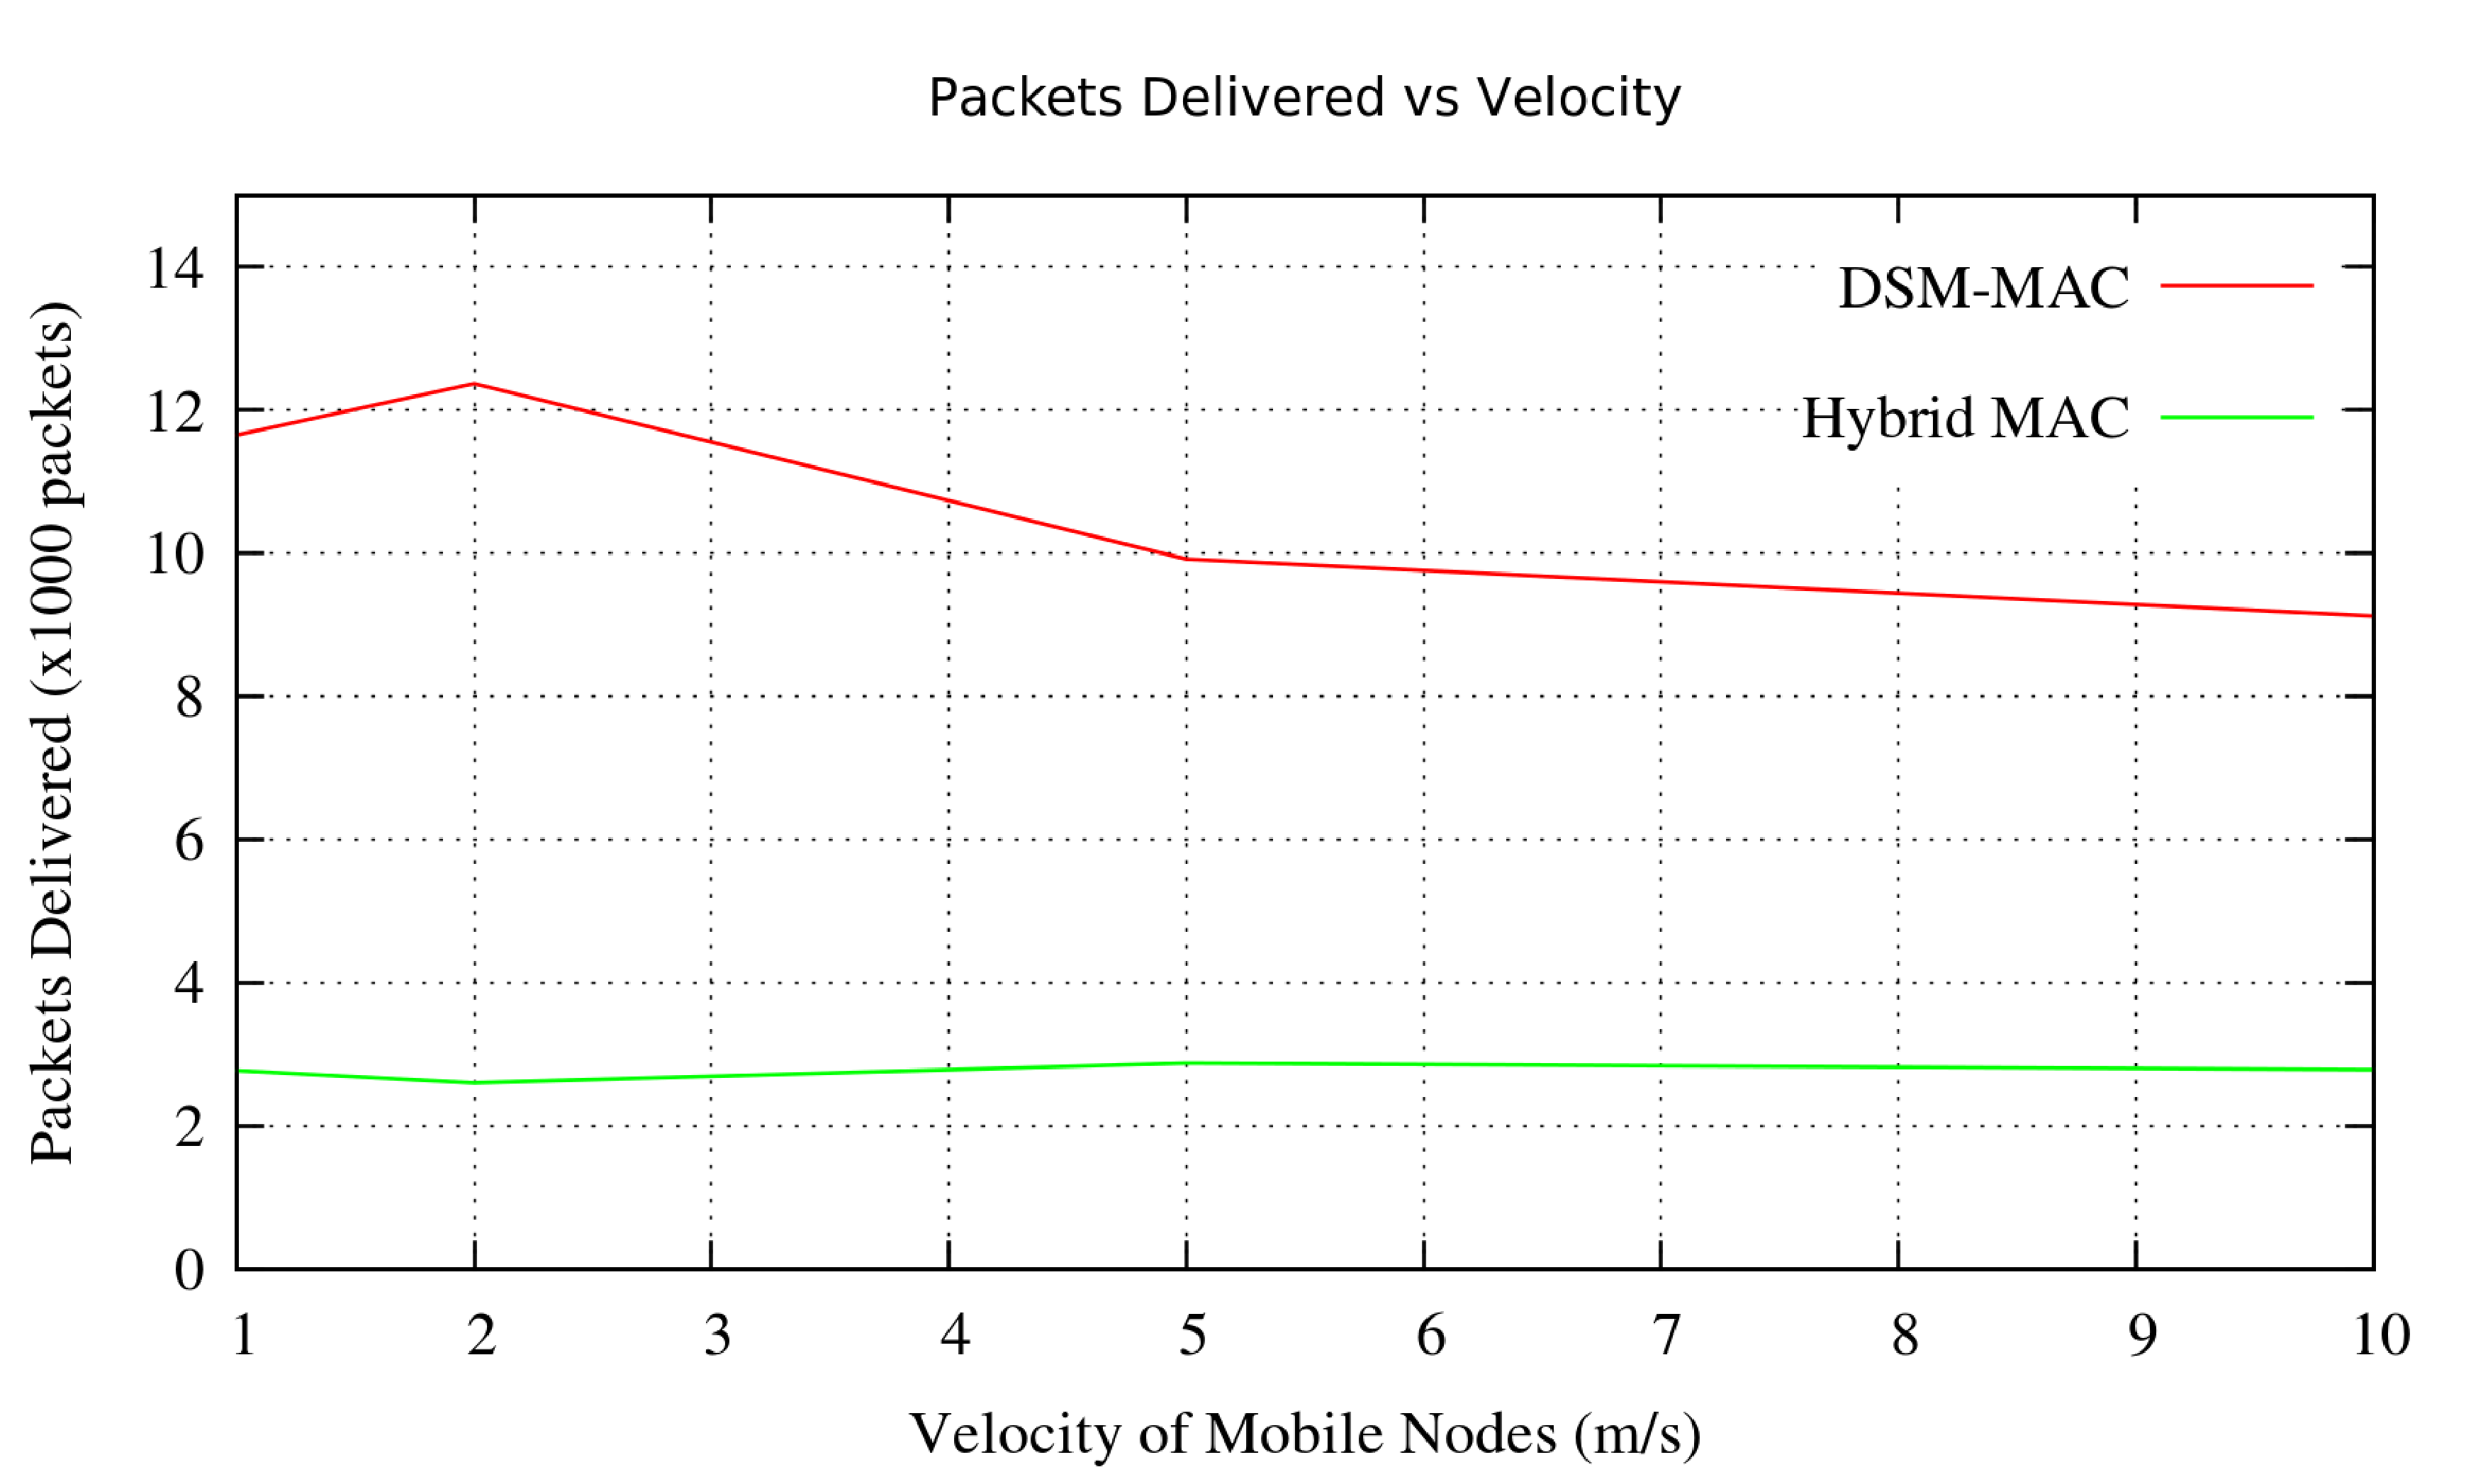
\includegraphics[ width=8.5cm,height=6cm]{pv}
  \end{center}
	\caption{Packets Delivered vs Velocity}
		\label{fig:pv}
\end{figure}
 
\begin{figure}[h]{} 
  \begin{center}
		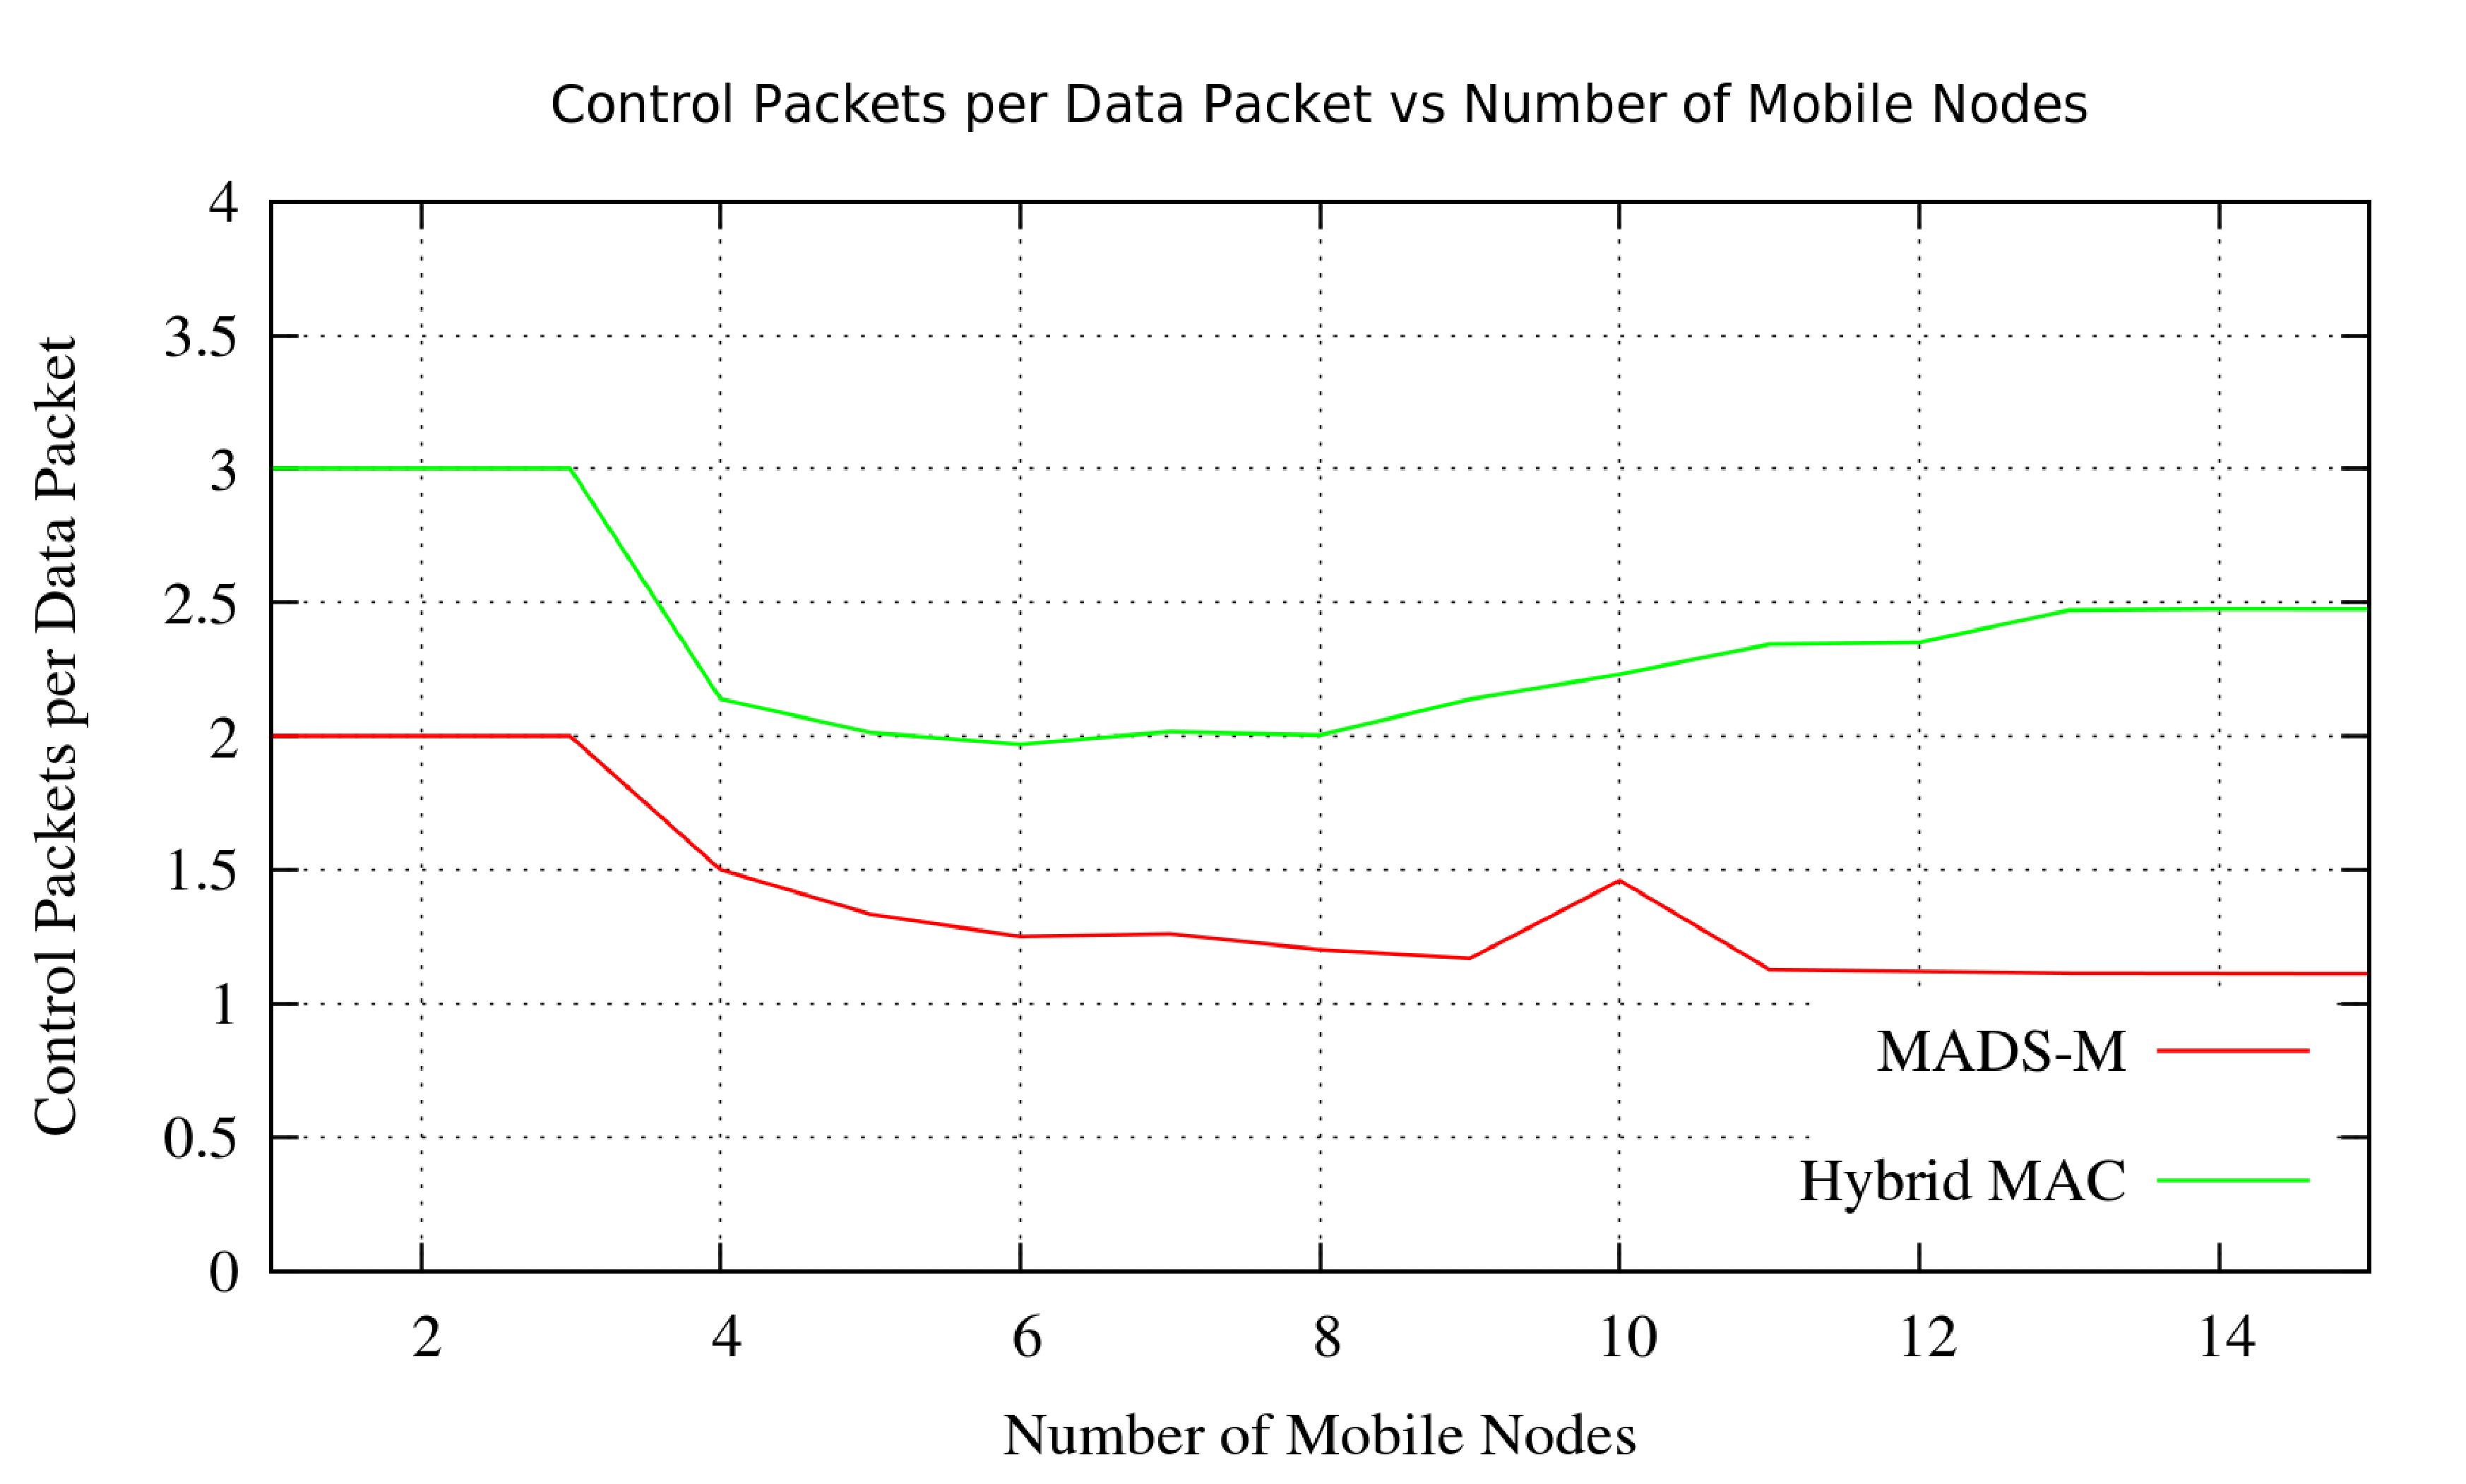
\includegraphics[ width=8.5cm,height=6cm]{cm}
  \end{center}
	\caption{Control Packets vs Number of Mobile Nodes}
		\label{fig:cm}
\end{figure}


The Communication overhead of the proposed protocol is compared with Hybrid MAC and is shown in the Figure \ref{fig:cm}. In this paper, we refer the communciation overhead to the number of control packets used for data communciation. The communication overhead is an essential factor affecting the overall network energy and the amount of channel interference in a network.  In WSN, more energy is spent on communication. If the communication overhead is high, then the overall energy spent for communication is also high. Also for single channel based MAC protocols, interference will be higher for higher communication overhead. Hence it is preferable to have a protocol with less communication overhead. Figure  \ref{fig:cm} plots the number of control packets used w.r.t the number of mobile nodes in a low mobility scenario. Simulation is done by changing the number of mobile nodes from $1$ to $15$. It is clear from Figure \ref{fig:cm} that the number of control packets generated in our approach is lower than that of Hybrid MAC.\\

In the above section, we have compared our approach with Hybrid MAC and have discussed the results based on packet delivery, packet delivery ratio, power consumption and the number of control packets. Even though our approach offers a slightly lower packet delivery ratio compared to Hybrid MAC, it should be noted that our approach performs better in terms of overall packets delivered, energy efficiency and the control overhead. 


\section{Scope}
